\documentclass[a4paper, 12pt, oneside, titlepage]{article}
\usepackage[T1]{fontenc}
\usepackage[utf8]{inputenc}
\usepackage[serbian]{babel}
\usepackage{mathptmx}
\usepackage{indentfirst}
\usepackage{titlesec}
\usepackage[left=1.5cm, right=1.5cm, top=2cm, bottom=2cm]{geometry}
\usepackage{mathtools}
\usepackage{graphicx}
\usepackage[export]{adjustbox}
\usepackage{fancyhdr}
\usepackage[titles]{tocloft}
\usepackage[nottoc,numbib]{tocbibind}
\usepackage{float}
\usepackage{xcolor, listings}
\usepackage{textcomp}
\usepackage{array}
\usepackage{textcomp}
\lstset{upquote=true}
\lstset{
basicstyle=\small\ttfamily,
columns=flexible,
breaklines=true
}

% Using Courier font
\renewcommand{\ttdefault}{pcr}

\titleformat{\section}
  {\Large\bfseries}{\thesection.}{1em}{}

\setcounter{tocdepth}{2}

%\renewcommand{\baselinestretch}{1.5} 

\renewcommand{\cftsecleader}{\cftdotfill{\cftdotsep}}

%\titlespacing{\section}{0pt}{0pt}{3*\bigskipamount}

\setlength{\headheight}{15pt}% ...at least 14,49998pt

\begin{document}
    \pagestyle{fancy}
    
    \renewcommand{\headrulewidth}{1pt}
    \renewcommand{\footrulewidth}{0pt}
    \fancyhf{}
    \lhead{\textit{Fakultet inženjerskih nauka, Kragujevac}}
    \rhead{\textit{Mikroprocesorski sistemi - projektna dokumentacija}}
    \rfoot{\thepage}
    
    \fancypagestyle{titlepage}
    {
	\fancyhf{}
	\renewcommand{\headrulewidth}{0pt}
	\renewcommand{\footrulewidth}{1pt}
	\cfoot{Kragujevac, Januar 2019.}
    }
    
    \begin{titlepage}
	\thispagestyle{titlepage}
	
	\begin{center}
	
	Univerzitet u Kragujevcu\\
	Fakultet inženjerskih nauka\\
	\vspace{50px}
	
\includegraphics[scale=2]{slike/logo}\\
	
	\vspace{160px}
	%\vfill
	
	\textbf{\huge Mikroprocesorski sistemi}\\
	\vspace{40px}
	{\LARGE Projektna dokumentacija:}\\
	\vspace{10px}
	{\Large Sistem dozvole lansiranja projektila iz tenka preko USART komunikacije}
	
	\end{center}
	
	\vfill
	
	\begin{minipage}{.3\textwidth}
	\begin{flushleft}
	    Student:\\
	    Aleksandar Kondić,
	    575/2015
	\end{flushleft}
	\end{minipage}
	\hfill
	\begin{minipage}{.25\textwidth}
	\begin{flushright}
	    Predmetni nastavnik:\\
	    Prof. dr Aleksandar Peulić\\
	\end{flushright}
	\end{minipage}
	\vspace{20px}
	
	\clearpage
	
    \end{titlepage}
    
    
    % Strana sa sadržajem
    \setcounter{page}{2}
    \tableofcontents
    \clearpage
    % Kraj strane sa sadržajem
    
%     \begin{figure}[ht]
%         \centering
%         \includegraphics[width=\textwidth]{slike/racun_primer}
%         \caption{Realni primer računa za gas - potencijalne lične i finansijske informacije su cenzurisane}
%         \label{fig:racun_primer} % Always put labels after captions...
%     \end{figure}
    
%     \section{Izjava o samostalnoj izradi rada (todo: stampaj, potpisi, skeniraj i zameni tekst sa slikom)}
%     \begin{center}
%       IZJAVA
%     \end{center}
%     
%     Potpisivanjem izavljujem da ja, Aleksandar Kondić, student Fakulteta inženjerskih nauka Univerziteta u Kragujevcu (broj indeksa: 575/2015), samostalno, uz konsultacije
%     sa predmetnim nastavnikom i korišćenjem literature koja je naznačena u projektnoj dokumentaciji, vršim izradu svog projektnog zadatka i dokumentacije iz predmeta Mikroprocesorski sistemi.
%     \bigbreak
%     \noindent Potpis: \_\_\_\_\_\_\_\_\_\_\_\_\_\_\_
%     \pagebreak
    
    \section{Izjava o samostalnoj izradi rada}
    \begin{center}
      
\includegraphics[width=\textwidth]{slike/scan}
      \label{fig:izjava_potpisana}
    \end{center}
    \pagebreak
    
    \section {Projektni zadatak}
    Na raznim delovima tenka postavljeni su senzori koji prate različite parametre tenka. Izlazi iz svih senzora su
    digitalni i jedine moguće vrednosti izlaza su logička jedinica (1 - 5V) ili logička nula (0 - 0V).
    
    Potrebno je napisati program za mikroprocesor koji je deo mikrokontrolera, koji korišćenjem USART komunikacije,
    omogućenom USART modulom mikrokontrolera u kojem se mikroprocesor nalazi, odgovara na zahteve spoljnjeg uređaja
    za lansiranje projektila iz cevi kupole tenka. Odgovor na zahtev zavisi od trenutnog stanja u kojem se tenk nalazi,
    koje je određeno vrednostima izlaza pomenutih senzora.
    
    Parametri tenka koji se razmatraju su:
    \begin{itemize}
      \item da li je zatvoren poklopac otvora vozača,
      \item da li je zatvoren poklopac otvora komandira,
      \item da li su zatvorena vrata nišandžije,
      \item da li su zatvorena vrata punjača,
      \item da li je cev oslobođena,
      \item da li je punjač slobodan, i
      \item da li tenk ima dozvolu za gađanje.
    \end{itemize}
    
    Ako je odgovor na neko od ovih pitanja ``da'', onda je logička vrednost na izlazu senzora koji meri odgovarajući
    parametar jednaka jedinici (1), u suprotnom je jednaka nuli (0).
    
      \subsection{Format zahteva i odgovora u USART komunikaciji}
      Format zahteva je jedan bajt koji ima heksadecimalnu vrednost 0x61.
      
      Mikrokontroler šalje odgovor samo ukoliko primljeni podatak odgovara napomenutom formatu zahteva. Format odgovora
      je takođe jedan bajt. Bit najmanje težine (bit 0 u ovom tekstu) predstavlja odgovor na zahtev za lansiranje
      projektila i logička vrednost 1 tog bita znači da tenk može da lansira projektil, dok logička vrednost 0 tog bita
      znači da tenk ne može da lansira projektil.
      
      Ostali bitovi u bajtu odgovora predstavljaju stanje ispunjenja uslova koje trenutno stanje tenka mora da ispuni
      da bi dobio dozvolu za lansiranje projektila. Ti uslovi su direktno povezani sa parametrima koje prate senzori na
      tenku, i \textbf{logička nula} u odgvoru znači da je odgovarajući uslov \textbf{ispunjen}, dok logička jedinica
      znači da odgovarajući uslov nije ispunjen. Sledi lista uslova kao i njihovo mapiranje na bitove bajta odgovora:
      \begin{itemize}
	\item \emph{bit 7 (\textbf{bit najveće težine} u ovom tekstu)} - zatvoren je poklopac otvora vozača,
	\item \emph{bit 6} - zatvoren je poklopac otvora komandira,
	\item \emph{bit 5} - zatvorena su vrata nišandžije,
	\item \emph{bit 4} - zatvorena su vrata punjača,
	\item \emph{bit 3} - cev je oslobođena,
	\item \emph{bit 2} - punjač je slobodan, i
	\item \emph{bit 1} - tenk ima dozvolu za gađanje.
      \end{itemize}
      
      Ovakav format odgovora ima specifično značenje. Ako su svi uslovi ispunjeni, vrednost bita 0 je logička jedinica
      dok su logičke vrednosti svih ostalih bitova nule, što predstavlja kod dozvolje za lansiranje projektila. Ako nisu
      svi uslovi ispunjeni, onda je vrednost bita 0 logička nula, dok svaki bit koji predstavlja uslov koji \emph{nije}
      ispunjen ima vrednost logičke jedinice. Ostali bitovi (bitovi koji odgovaraju uslovima koji su ispunjeni), naravno,
      imaju vrednost logičke nule.
      
    \section{Tehnički opis sistema} \label{sec:techspec}
    \noindent Tokom izrade ovog projektnog zadatka korišćene su sledeće tehničke komponente:
    \begin{itemize}
      \item Razvojno okruženje EasyMx PRO\texttrademark{} v7 for STM32\textsuperscript{\textregistered}
      \item EasyMx PRO\texttrademark{} v7 for STM32\textsuperscript{\textregistered} MCUcard with STM32F476VGT6
    \end{itemize}
    
    \noindent Vredi napomenuti i softverske komponente koje su korišćene tokom izrade ovog projektnog zadatka:
    \begin{itemize}
      \item mikroC PRO for ARM
      \item mikroProg Suite for ARM
    \end{itemize}
    
      \subsection{Razvojno okruženje EasyMx PRO\texttrademark{} v7 for STM32\textsuperscript{\textregistered}}
      EasyMx PRO v7 for STM32 ARM® je razvojno okruženje za STM32 ARM uređaje. Sadrži široki spektar modula i
      ulazno/izlaznih elemenata koji su pogodni kao korisnički interfejs prema mikrokontroleru, koji je koristan
      prilikom projektovanja i razvoja mikroprocesorskih sistema.
      \bigbreak
      \noindent Tehnička specifikacija:
      \bigbreak
      \begin{tabular}{>{\bfseries}p{0.237\linewidth}p{0.678\linewidth}}
	Primena: & Razvoj i testiranje \emph{firmware}-a, kreiranje prototipova, učenje o programiranju \emph{embedded}
	sistema \\
	Veličina displeja: & 2.8'' \\
	Rezolucija: & 320x240px \\
	Grafički kontroler: & Ugrađen unutar MCU kartice \\
	Ekran osetljiv na dodir: & Rezistivni \\
	Arhitektura: & ARM (32-bitna) \\
	MCU: & MCU sa mikrokontrolerom STM32F476VGT6 \\
	Moduli: & Priključci za LM35 i DS1820 senzore temperature, džojstik, ADC potenciometri \\
	Programator: & mikroProg for STM32 \\
	Skladištenje podataka: & Serijska FLASH memorija, serijski EEPROM (1024 bajtova), slot za microSD karticu \\
	Zvuk i audio: & Piezo buzzer, VS1053 MPEG Audio codec, Audio konektori \\
	Proširivost: & 2 x mikroBUS priključka, 2 x IDC10 zaglavlja za svaki PORT \\
	Integrisanje: & montažne rupe \\
	Napajanje: & 5V preko USB-a ili 9-32V AC, 7-23V DC preko adaptera \\
      \end{tabular}
      \begin{figure}[H]
        \centering
        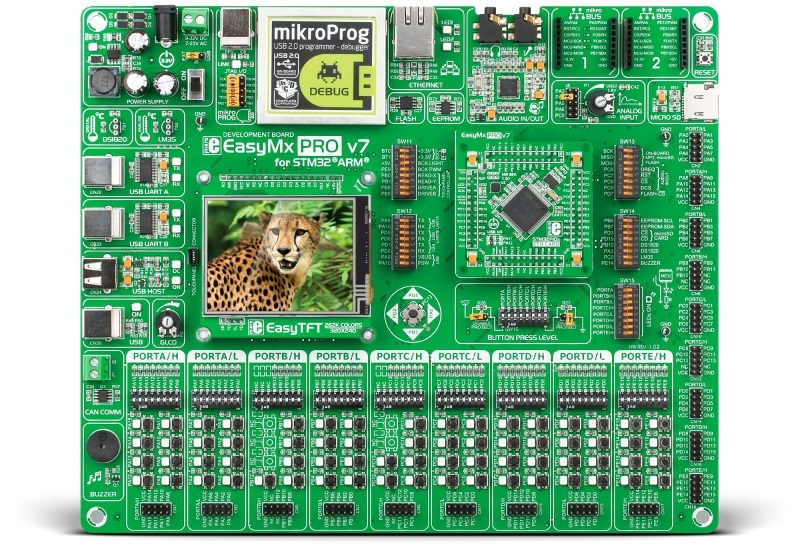
\includegraphics[width=\textwidth]{slike/easymx}
        \caption{Razvojno okruženje EasyMX PRO\texttrademark{} v7 for STM32\textsuperscript{\textregistered}}
        \label{fig:easymx} % Always put labels after captions...
      \end{figure}
      
      \subsection{EasyMx PRO\texttrademark{} v7 for STM32\textsuperscript{\textregistered} MCUcard with STM32F746VGT6}
      MCU kartica je modul razvojnog okruženja koja služi za povezivanje mikrokontrolera sa razvojnim okruženjem.
      Ovo je prva MCU kartica za EasyMx PRO v7 koja nosi ARM® Cortex®-M7 mikrokontroler. Ova MCU kartica na sebi
      ima STM32F746-100 mikrokontroler sa periferijama koje se nalaze na čipu. Takođe sadrži kristalni oscilator
      frekvencije od 25 MHz, USB komunikacione linije i Ethernet primopredajnik.
      \bigbreak
      \noindent Tehnička specifikacija:
      \bigbreak
      \begin{tabular}{>{\bfseries}p{0.2\linewidth}p{0.7\linewidth}}
	Arhitektura: & ARM (32-bitna) \\
	MCU: & STM32F476VGT6 \\
	Brzina MCU: & 462 DMIPS, 216 MHz, 2.14 DMIPS/MHz \\
	Napajanje: & 3.3V \\
	Kompatibilnost sa: & EasyMx PRO v7 for STM32 \\
      \end{tabular}
      \begin{figure}[H]
	\centering
	\begin{minipage}{0.45\textwidth}
	    \centering
	    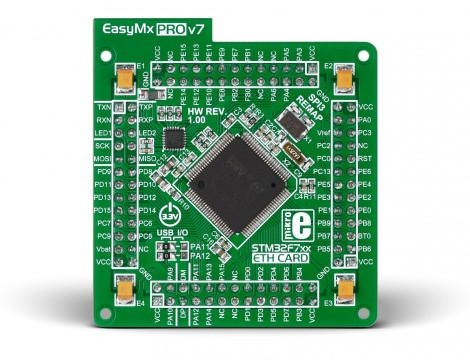
\includegraphics[width=0.9\textwidth]{slike/stm32_mcu} % first figure itself
	    \caption{MCU kartica sa STM32F746VGT6 mikrokontrolerom}
	    \label{fig:stm32_mcu} % Always put labels after captions...
	\end{minipage}\hfill
	\begin{minipage}{0.45\textwidth}
	    \centering
	    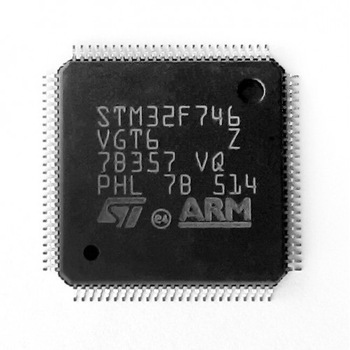
\includegraphics[width=0.9\textwidth]{slike/stm32} % second figure itself
	    \caption{STM32F746VGT6 mikrokontroler}
	    \label{fig:stm32} % Always put labels after captions...
	\end{minipage}
      \end{figure}
      
      \subsection{mikroC PRO for ARM}
      mikroC PRO for ARM je integrisano softversko razvojno okruženje za programiranje mikroprocesora ARM arhitekture u programskom jeziku C - sa ponekim modifikacijama programskog jezika
      od srane Mikroelektronike. U sebi takođe sadrži mikrC Pro programski prevodilac za ARM mikrokontrolere/uređaje. Za izradu ovog projekta bila je dovoljna besplatna (demo) verzija
      programa zbog male veličine rezultujućeg programskog koda za mikroprocesor.
      
      \noindent Sledi lista ponekih karakterističnosti ovog razvojnog okruženja softvera:
      \begin{itemize}
	\item Preko 1200 funkcija iz ugrađenih biblioteka
	\item Preko 400 primera programskog koda za različite podržane uređaje
	\item Preko 1140 podržanih mikrokontrolera
	\item FreeRTOS podrška za razvoj sistema koji rade u realnom vremenu
	\item Visual TFT integrisano razvojno okruženje za razvoj grafičkih aplikacija
	\item Hardware debugging
	\item Obimna dokumentacija
	\item Doživotna licenca
      \end{itemize}
      \begin{figure}[H]
        \centering
        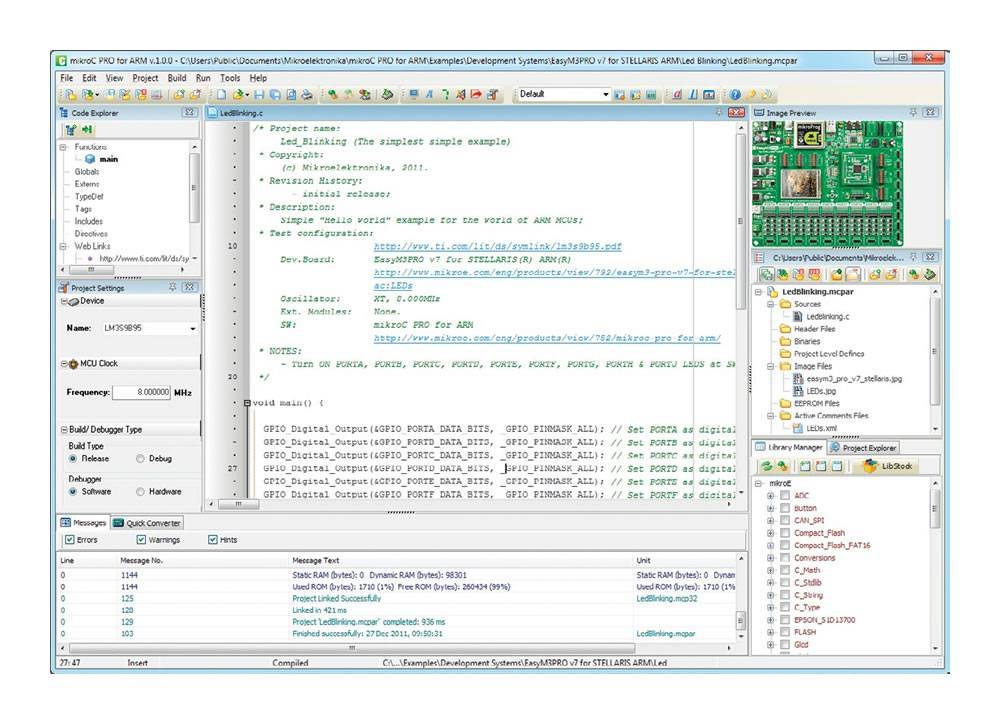
\includegraphics[width=\textwidth]{slike/mikroc_pro_arm_ide}
        \caption{mikroC PRO for ARM softversko razvojno okruženje}
        \label{fig:mikroc_pro_arm_ide} % Always put labels after captions...
      \end{figure}
      
      \subsection{mikroProg Suite for ARM}
      \begin{figure}[H]
      \noindent\begin{minipage}[t]{0.7\textwidth}
	\emph{mikroProg Suite} je softver koji se koristi za upravljanje programatorom razvojnog okruženja - bio on ugrađen kao komponenta razvojnog okruženja ili eksterna komponenta.
	On je ključan deo programiranja mikrokontrolera kodom koji je generisao programski prevodilac. Takođe omogućava upravljanje kodom i podacima posle procesa programiranja
	mikrokontrolera. Interfejs ove aplikacije prikazan je na slici \ref{fig:mikroprog_suite_arm}.
      \end{minipage}%
      \hfill%
      \begin{minipage}[t]{0.3\textwidth}
	\centering
	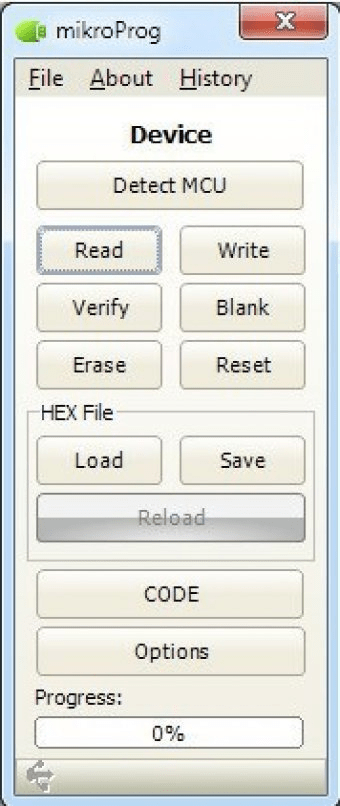
\includegraphics[scale=0.27, valign=t]{slike/mikroprog_suite_arm}
	\caption{mikroProg Suite for ARM}
	\label{fig:mikroprog_suite_arm} % Always put labels after captions...
      \end{minipage}%
      \end{figure}
    
    \section{Tehnički uslovi}
    U realnoj praktičnoj primeni ovog sistema, neće biti korišćeni ni EasyMx razvojno okružene, niti MCU kartica na kojoj se nalazi mikrokontroler sa dodatnim periferijama, već će se samo
    koristiti mikrokontroler (STM32F476VGT6). Iz navedenog sledi da tehnički uslovi sistema zavise isključivo od tehničkih uslova samog mikrokontrolera.
    
      \subsection{Maksimalne ocene tehničkih uslova uređaja}
      Slede apsolutno maksimalni operativni i skladišni uslovi mikrokontrolera, gde prekoračenje ograničenja koji slede u najvećem broju slučajeva rezultuje u oštećenju samog mikrokontrolera:
      \begin{itemize}
	\item \textbf{Naponski uslovi}:
	\begin{itemize}
	  \item Napajanje: $-0.3 V \le V_{DD} \le 4 V$
	  \item Napon na ulaznim pinovima: $-0.3 V \le V_{IN} \le 4 V$
	\end{itemize}
	\item \textbf{Strujni uslovi}:
	\begin{itemize}
	\item $I_{V_{DD}}max = 100 mA$ --- Maksimalna jačina struje jedne dovodne linije napajanja
	\item $I_{V_{SS}}max = -100 mA$ --- Maksimalna jačina struje jedne odvodne linije napajanja (uzemljena linija)
	\item $|I_{IO}max| = 25mA$ --- Maksimalna jačina struje koju ulazno/izlazni pin šalje ili prima
	\item $\max \sum I_{V_{DD}} = 320 mA$ --- Maksimalna jačina ukupne dovodne struje napajanja
	\item $\max \sum I_{V_{SS}} = -320 mA$ --- Maksimalna jačina ukupne odvodne struje napajanja
	\end{itemize}
	\item \textbf{Termički uslovi}:
	\begin{itemize}
	  \item $-65 $\textdegree$C \le T_{STG} \le 150 $\textdegree$C$ --- Opseg temperature okruženja u kojem uređaj može da se skladišti bez njegovog rada
	  \item $T_{Jmax} = 125 $\textdegree$C$ --- Maksimalna radna temperatura poluprovodničkih komponenti uređaja
	\end{itemize}
      \end{itemize}
      
      \subsection{Generalni operativni uslovi uređaja}
      U sledećoj listi su opisani opsezi parametara mikrokontrolera koji su tipični za takav mikrokontroler tokom njegovog rada:
      \begin{itemize}
	\item $1.7 V \le V_{DD} \le 3.3V$ --- Operativni opseg napajanja mikrokontrolera
	\item $-0.3V \le V_{IN} \le 3.3V$ --- Operativni opseg napona na ulaznim pinovima
	\item $P_{Dmax} = 351 mW$ --- Maksimalna disipacija snage
	\item $-40 $\textdegree$C \le T_{J} \le 125 $\textdegree$C$ --- Opseg operativne temperature poluprovodničkih elemenata
      \end{itemize}
      
      \noindent Neka od ovih ograničenja se tehnički mogu prekoračiti, ali samo uz oprez.
    
    \pagebreak
    \section{Prilog o primenjenim propisanim merama zaštite na radu u skladu sa Zakonom o bezbednosti i zdravlju na radu}
    Prilikom izrade projektnog zadatka ispoštovana su bezbednosna pravila koja su u skladu sa Zakonom o bezbednosti i zdravlju na radu („Sl. glasnik RS“, br. 101/2005).
    \pagebreak
    
    \section{Predmer i predračun radova i materijala}
    Uzeće se u obzir samo materijali koji su potrebni za realizaciju ovog projektnog zadatka, izuzimajući elemente koji su spoljni u odnosu na realizovani sistem, kao što su senzori,
    potrebno kabliranje, uređaj koji šalje zahteve mikrokontroleru preko USART komunikacije, i sam tenk čiji se parametri mere. Takođe će se izostaviti cena vršenja razvoja samog
    sistema (rada), zato što je on u ovom slučaju praktično besplatan.
    \bigbreak
    \noindent Slede materijali koji su bili potrebni za izradu projektnog zadatka, zajedno sa njihovim cenama:
    \begin{itemize}
      \item Razvojno okruženje EasyMx PRO\texttrademark{} v7 for STM32\textsuperscript{\textregistered}: \textbf{169.00 USD} $\approx$ \textbf{17457.99 RSD}
      \item EasyMx PRO\texttrademark{} v7 for STM32\textsuperscript{\textregistered} MCUcard with STM32F476VGT6: \textbf{39.00 USD} $\approx$ \textbf{4028.77 RSD}
      \item \textbf{Ukupno}: 208.00 USD $\approx$ 21486,76 RSD
    \end{itemize}
    \bigbreak
    Treba napomenuti da su cene naznačenih proizvoda preuzete sa zvanicne internet prezentacije Mikroelektronike u valuti \emph{USD} i konvertovane u valutu \emph{RSD} koristeći kursnu
    listu Narodne banke Srbije, sve u trenutku izrade projektne dokumentacije.
    
    \section{Specifikacija materijala}
    Pošto su svi materijali koji su korišćeni prilikom izrade ovog projektnog zadatka zapravo tehnički moduli, a tehničke specifikacije tih modula su naznačene u odeljku \ref{sec:techspec},
    u ovom odeljku navedene su dimenzije materijala sa slikama.
    \bigbreak
    \noindent Dimenzije MCU kartice: 55.88mm x 61.09mm
    \begin{figure}[H]
        \centering
        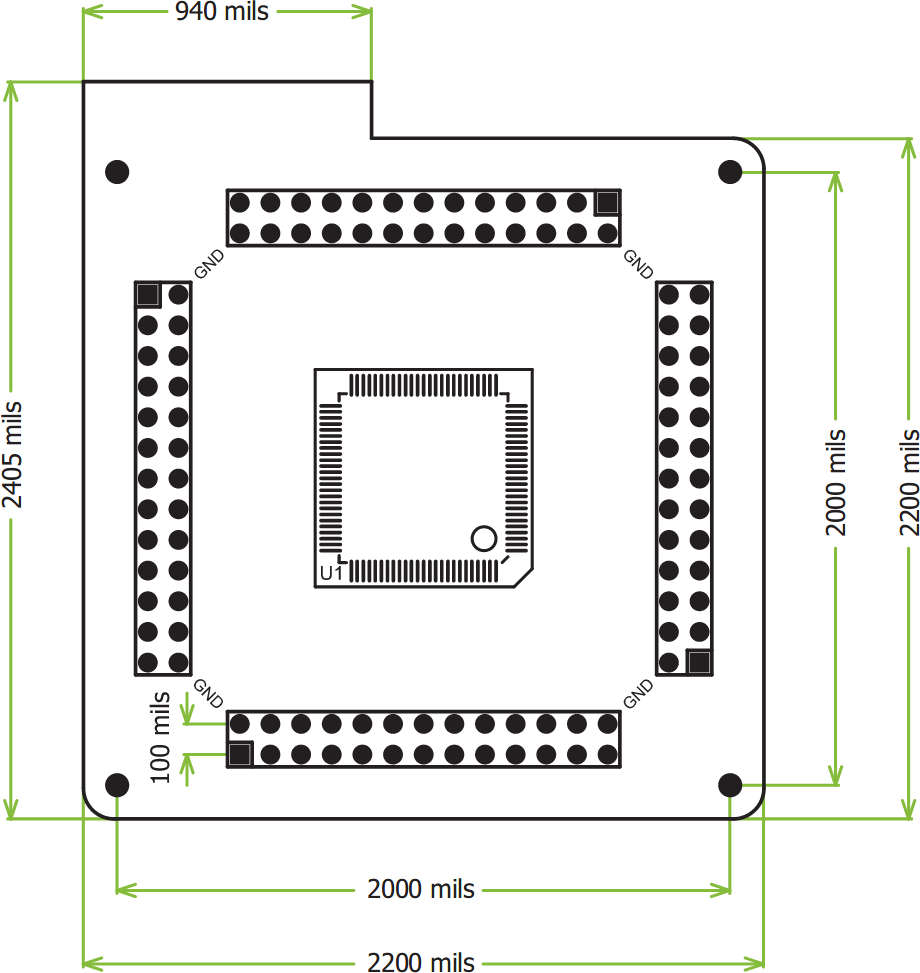
\includegraphics[width=0.5\textwidth]{slike/dim_mcu_card}
        \caption{MCU kartica}
        \label{fig:dim_mcu_card} % Always put labels after captions...
    \end{figure}
    \pagebreak
    
    \noindent Dimenzije EasyMx Pro v7 razvojnog okruženja: 28.83cm x 24.76cm
    \begin{figure}[H]
        \centering
        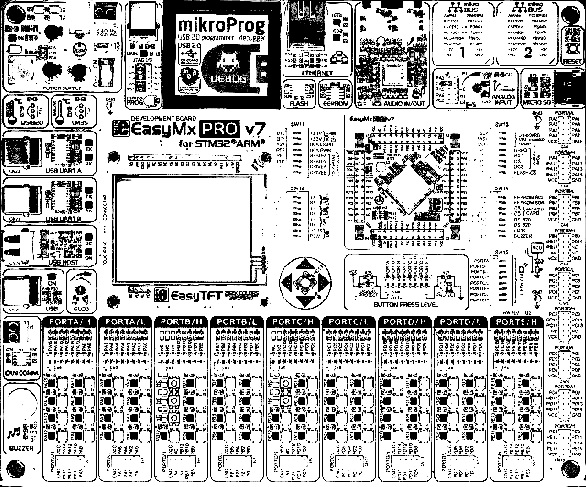
\includegraphics[width=\textwidth]{slike/dim_easymx}
        \caption{EasyMx Pro v7}
        \label{fig:dim_easymx} % Always put labels after captions...
    \end{figure}
    
    \section{Potrebni odgovarajući proračuni}
    Prilikom izrade ovog projekta nisu vršeni nikakvi proračuni u kontektsu izbora komponenti i fizičkih veličina. Realizacija projektnog zadatka bavila se isključivo logičkim vrednostima
    na digitalnim pinovima.
    
    Možda vredi napomenuti bitovske operacije koje se izvršavaju nad logičkim vrednostima ulaza koji su povezani sa senzorima, radi dobijanja vrednosti bajta odgovora, koji se šalje pomoću
    USART komunikacije pri zahtevu od spoljnjeg uređaja. Pošto se svi ulazni pinovi mikrokontrolera koji su povezani sa senzorima nalaze na nižem delu porta D - PORTD/L - vrednosti sa
    svih senzora dostupni su u okviru jednog bajta koji predstavlja PORTD/L u programu. Pošto su viši bitovi odgovora na zahtev zapravo invertovani bitovi ulaza (PORTD/L), dovoljno je
    invertovati vrednost bajta koji predstavlja ulaze na PORTD/L, a bit najmanje težine postaviti u skladu sa ispunjenjem svih uslova tenka za lansiranje projektila, da bi se izračunala
    vrednost odgovora na zahtev. Ovaj način računanja odgovora na zahtev prikazan je u sledećem listingu:
    \lstinputlisting[
           language=C,
           showspaces=false,
           basicstyle=\ttfamily,
           numbers=left,
           numberstyle=\tiny,
           commentstyle=\color{gray}
        ]{snippet.c}
    
    \section{Odgovarajuća grafička dokumentacija}
      \subsection{Šema povezivanja senzora, mikrokontrolera i spoljnjeg uređaja koji šalje zahteve}
      \begin{figure}[H]
        \centering
        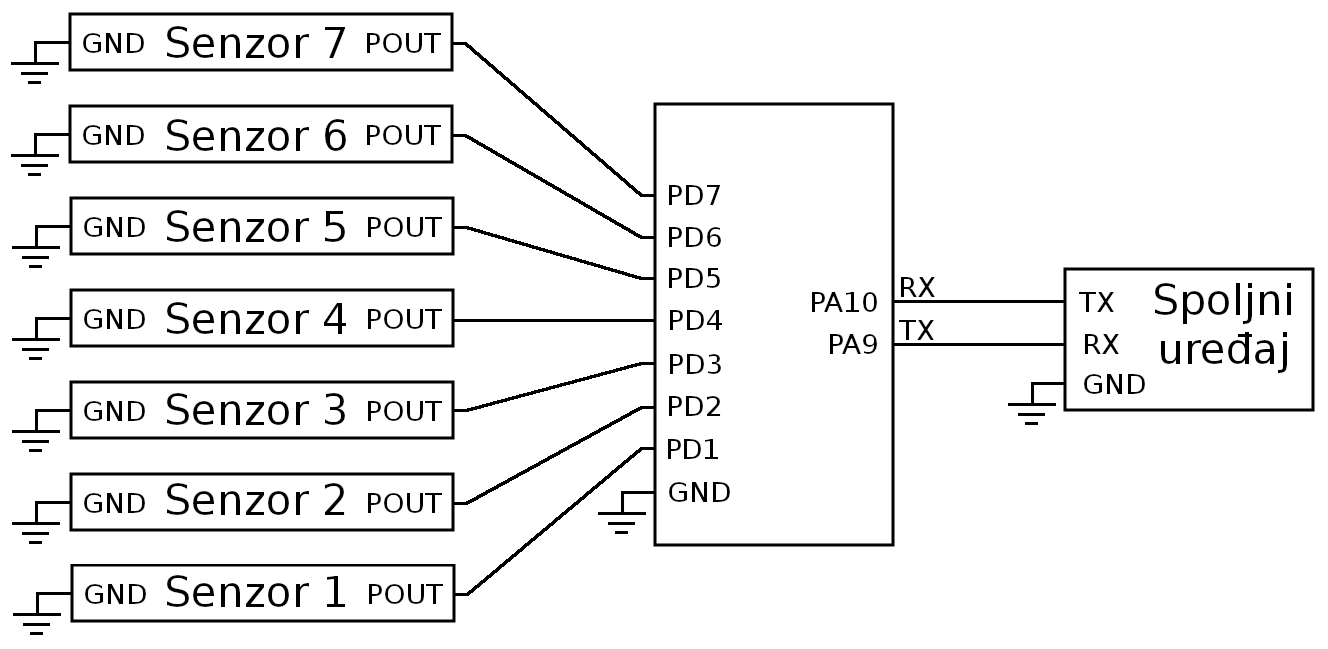
\includegraphics[width=\textwidth]{slike/povezivanje}
        \caption{Šema povezivanja senzora, mikrokontrolera i spoljnjeg uređaja koji šalje zahteve i prima odgovore}
        \label{fig:povezivanje} % Always put labels after captions...
      \end{figure}
      
      Svaki od senzora na šemi prati po jedan od navedenih parametara tenka. U kontekstu odgovora koji mikrokontroler šalje spoljnom uređaju, redosled ovih senzoran nije ni bitan,
      ali bi redosled trebao da bude specifičan da bi se pokoravao preciznoj definiciji projektnog zadatka, gde je naznačeno koji bit ulaznog registra predstavlja koji parametar
      tenka.
      
      \subsection{Relevantne blok šeme mikrokontrolera}
      \begin{figure}[H]
        \centering
        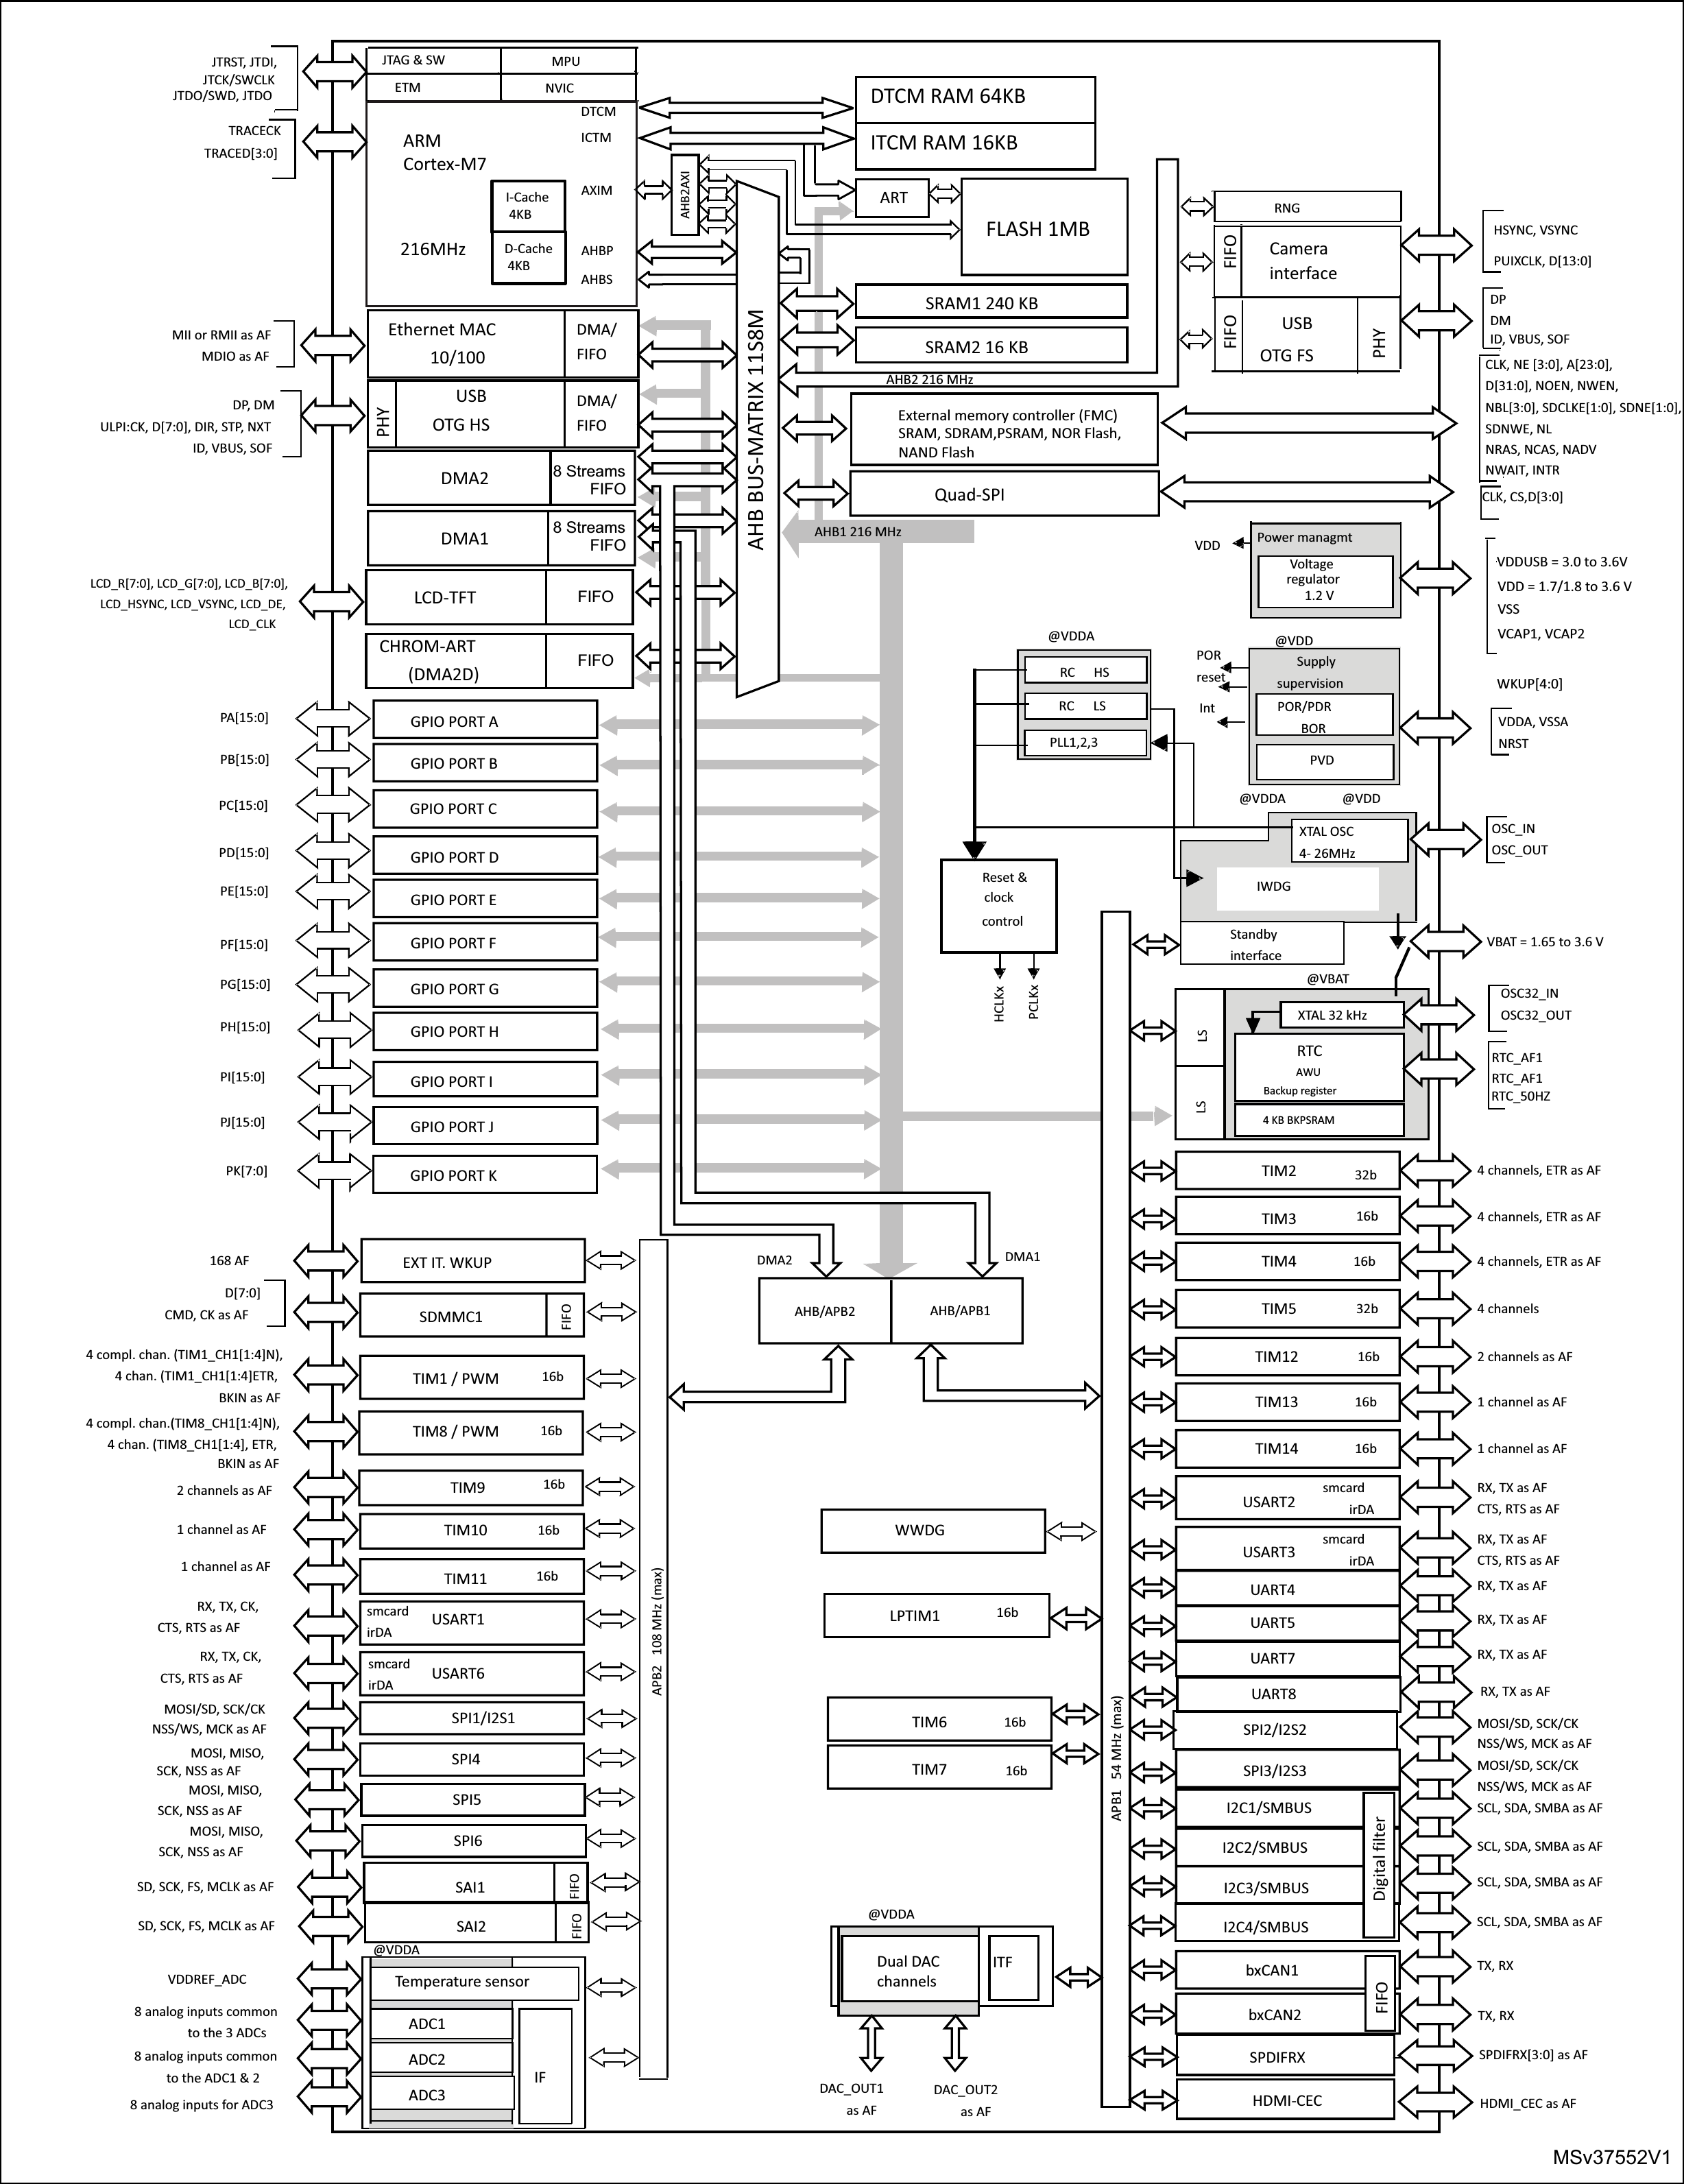
\includegraphics[height=0.9\textheight]{slike/blok_mikrokontroler}
        \caption{Blok šema mikrokontrolera STM32F476VGT6}
        \label{fig:blok_mikrokontroler} % Always put labels after captions...
      \end{figure}
      
      \begin{figure}[H]
        \centering
        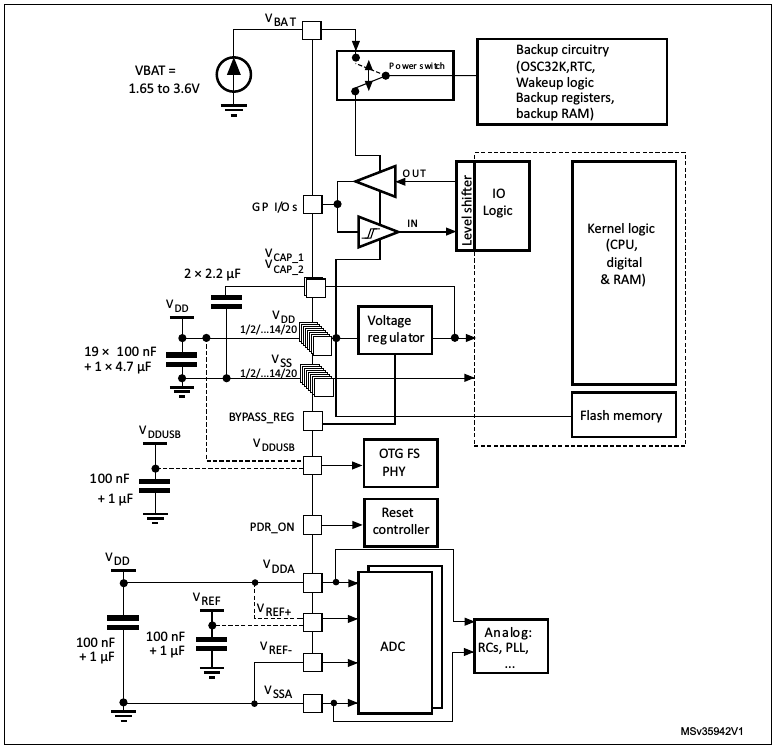
\includegraphics[width=\textwidth]{slike/blok_napajanje}
        \caption{Šema napajanja za mikrokontroler STM32F476VGT6}
        \label{fig:blok_napajanje} % Always put labels after captions...
      \end{figure}
      
      \begin{figure}[H]
        \centering
        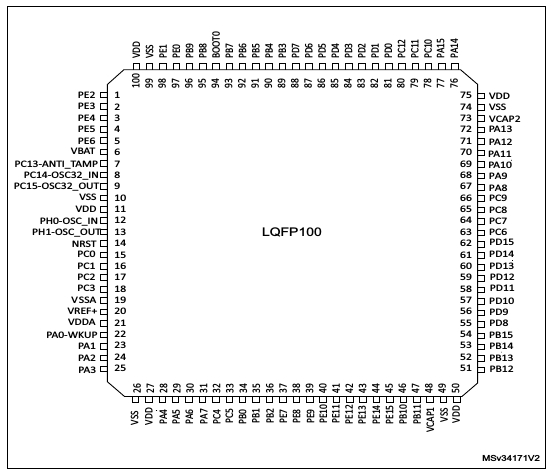
\includegraphics[width=\textwidth]{slike/blok_pinovi}
        \caption{Pinovi na mikrokontroleru STM32F476VGT6}
        \label{fig:blok_pinovi} % Always put labels after captions...
      \end{figure}
    
    
    \clearpage
    \begin{thebibliography}{4}
        \bibitem{easymx}
        EasyMx Pro v7 na sajtu Mikroelektronike (\today):\\
	\lstinline|https://www.mikroe.com/easymx-pro-stm32|
        
        \bibitem{mcu_card}
        MCU kartica sa mikrokontrolerom STM32F476VGT6 na sajtu Mikroelektronike (\today):\\
	\lstinline|https://www.mikroe.com/easymx-pro-v7-stm32-stm32f746vgt6|
	
	\bibitem{datasheet}
	Datasheet za mikrokontroler STM32F476VGT6 (\today):\\
	\lstinline|https://www.st.com/resource/en/datasheet/stm32f746vg.pdf|
	
	\bibitem{mikroc}
	mikroC PRO for ARM (\today):\\
	\lstinline|https://www.mikroe.com/mikroc-arm|
	
	\bibitem{mikroc_gpio}
	GPIO biblioteka za mikroC (\today):\\
	\lstinline|http://download.mikroe.com/documents/compilers/mikroc/arm/help/gpio_library.htm|
	
	\bibitem{mikroc_UART}
	UART biblioteka za mikroC (\today):\\
	\lstinline|http://download.mikroe.com/documents/compilers/mikroc/arm/help/uart_library.htm|
	
	\bibitem{zakon}
	Zakon o bezbednosti i zdravlju na radu (\today):\\
	\lstinline|http://www.minrzs.gov.rs/files/doc/bezbednost/zakon%20o%20bezbednosti%20i%20zdravlju%20na%20radu.pdf|
        
	\bibitem{kursna_lista_nbs}
	Kursna lista Narodne banke Srbije (\today):\\
	\lstinline|https://www.kursna-lista.com/kursna-lista-nbs|
    \end{thebibliography}
    \clearpage
    
    

    
    
\end{document}

